%% %% %% %%
%%
%% Parte A de la práctica
%%
%% %% %% %%

\documentclass[../procedimientos.tex]{subfiles}
\graphicspath{{\subfix{../../images/}}}

\begin{document}
\subsection{Parte A}
\subsubsection{Instrucciones}
Diseñe un circuito digital con compuertas que funcione de la siguiente forma:
Cuando $C$ se coloca en bajo se debe detectar y señalizar, con un diodo led de 
color verde, todos los números divisibles entre cuatro; el led rojo no debe 
encender. Si $C$ cambia a un nivel alto, entonces se debe detectar y 
señalizar, con un led de color rojo, todos los números divisibles entre tres 
y, además, con el led verde, los números divisibles por cinco. El conjunto de 
números es de 4 bits.
\begin{figure}[H]
  \centering
  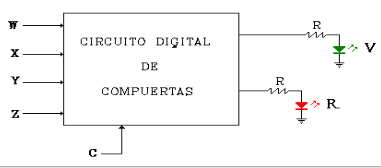
\includegraphics[width=0.5\textwidth]{a_instruction}
  \caption{Ejercicio A}
  \label{fig:a_inst}
\end{figure}

\subsubsection{Análisis}\label{subs:analisis_a}
Antes de comenzar a diseñar la solución para este problema, se requiere 
obtener una función lógica que describa el comportamiento indicado en la 
descripción del problema. Para esto, se asumirá que las funciones buscadas son 
$R(cwxyz)$ para el LED rojo y $V(cwxyz)$ para el LED verde; la cadena $cwxyz$ 
es la representación en bits del número a identificar. El análisis se puede 
comenzar a través de las tablas de verdad de las funciones solicitadas; sin 
embargo, se necesitarían analizar las 32 posibles combinaciones para las 
entradas. Se optó por deducir las formas canónicas \textit{SOP} (Suma de 
Productos, por sus siglas en inglés) de forma inmediata con los casos de 
solicitados.

Primero, para el caso del LED verde, se tienen que marcar todos los 
\textbf{números divisibles entre cuatro} que tienen $C=0$. Los números a 
anlizar son exclusivamente: $0$, $4$, $8$, $12$. De igual forma, se deben 
marcar los \textbf{números divisibles entre cinco} que tienen $C=1$, los 
cuales se listan a continuación: $20$, $25$ y $30$. Con esto, la forma normal 
\textit{SOP} se puede deducir de la siguiente forma:
\begin{equation*}
  V(cwxyz) = \sum_m (0, 4, 8, 12, 20, 25, 30)
\end{equation*}

Desarrollando la suma de productos para simplificar la expresión, se tiene:
\begin{align*}
  V(cwxyz) &= \nt{c}\nt{w}\nt{x}\nt{y}\nt{z} + \nt{c}\nt{w}x\nt{y}\nt{z} + 
  \nt{c}w\nt{x}\nt{y}\nt{z} + \nt{c}wx\nt{y}\nt{z} + c\nt{w}x\nt{y}\nt{z} + 
  cw\nt{x}\nt{y}z + cwxy\nt{z}\\
  &= \nt{c}\nt{y}\nt{z} (\nt{w}\nt{x} + \nt{w}x + w\nt{x} + wx) + 
  c\nt{w}x\nt{y}\nt{z} + cw\nt{x}\nt{y}z + cwxy\nt{z}\\
  &= \nt{c}\nt{y}\nt{z} (1) + c\nt{w}x\nt{y}\nt{z} + cw\nt{x}\nt{y}z + 
  cwxy\nt{z}\\
  &= \nt{c}\nt{y}\nt{z} + c\nt{w}x\nt{y}\nt{z} + cw\nt{x}\nt{y}z + 
  cwxy\nt{z}\\
  &= \nt{c}\nt{y}\nt{z} + c\nt{w}x\nt{y}\nt{z} + cw\nt{x}\nt{y}z + 
  cwxy\nt{z}\\
  &= \nt{c}\nt{y}\nt{z} + cx\nt{z} (\nt{w}\nt{y} + wy) + cw\nt{x}\nt{y}z\\
  &= \nt{c}\nt{y}\nt{z} + cx\nt{z} (w \odot y) + cw\nt{x}\nt{y}z
\end{align*}
\begin{equation*}
  \boxed{
    \therefore V(cwxyz) = \nt{c}\nt{y}\nt{z} + cx\nt{z} (w \odot y) + 
  cw\nt{x}\nt{y}z
  }
\end{equation*}

Por otra parte, para el caso del LED rojo, se tienen que marcar todos los 
\textbf{números divisibles entre tres} que tienen $C=1$, la lista se muestra a 
continuación: $18$, $21$, $24$, $27$ y $30$. Con esto, es posible colocar 
$R(cwxyz)$ en su forma canónica \textit{SOP}, tal como se muestra a 
continuación:
\begin{equation*}
  R(cwxyz) = \sum_m (18, 21, 24, 27, 30)
\end{equation*}

Desarrrollando la suma de productos para simplificar la expresión, se tiene:
\begin{align*}
  R(cwxyz) &= c\nt{w}\nt{x}y\nt{z} + c\nt{w}x\nt{y}z + cw\nt{x}\nt{y}\nt{z} + 
  cw\nt{x}yz + cwxy\nt{z}\\
  &= c(\nt{w}\nt{x}y\nt{z} + \nt{w}x\nt{y}z + w\nt{x}\nt{y}\nt{z} + w\nt{x}yz 
  + wxy\nt{z})\\
  &= c(\nt{x}\nt{z}(\nt{w}y + x\nt{y}) + \nt{w}x\nt{y}z + w\nt{x}yz + 
  wxy\nt{z})\\
  &= c(\nt{x}\nt{z}(\nt{w}y + x\nt{y}) + \nt{w}x\nt{y}z + wy(\nt{x}z + 
  x\nt{z}))\\
  &= c(\nt{x}\nt{z}(w \oplus y) + \nt{w}x\nt{y}z + wy(x \oplus z))
\end{align*}
\begin{equation*}
  \boxed{
    \therefore R(cwxyz) = c(\nt{x}\nt{z}(w \oplus y) + wy(x \oplus z) + 
    \nt{w}x\nt{y}z)
  }
\end{equation*}

\subsubsection{Implementación en Quartus}\label{subs:a_imp}
La implementación en la plataforma \textit{Quartus II} del sistema anterior se 
dividió en símbolos separados. Por un lado, se tiene el símbolo referente a 
$f_v$, y por otro se tiene $f_r$. Cada uno de ellos toma como entrada al 
arreglo $Ent$, la cual asigna los valores correspondientes a las variables 
$c$, $w$, $x$, $y$ y $z$ de la siguiente forma:
\begin{itemize}
  \item $Ent[4] \Rightarrow c$
  \item $Ent[3] \Rightarrow w$
  \item $Ent[2] \Rightarrow x$
  \item $Ent[1] \Rightarrow y$
  \item $Ent[0] \Rightarrow z$
\end{itemize}

Los diagrámas de bloques se pueden ver a continuación:
\begin{figure}[H]
  \centering
  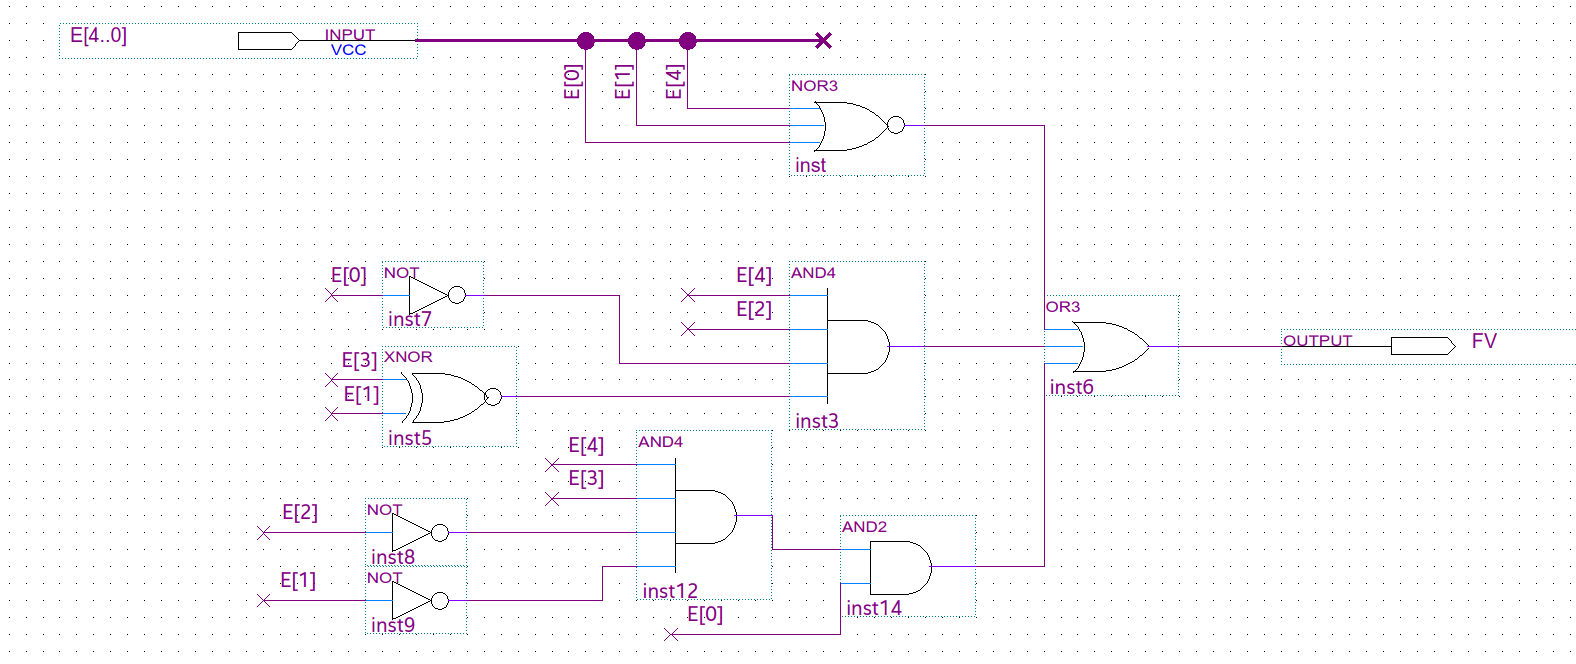
\includegraphics[width=\textwidth]{a_fv}
  \caption{Implementación de $f_v(cwxyz)$}
  \label{fig:a_fv}
\end{figure}
\begin{figure}[H]
  \centering
  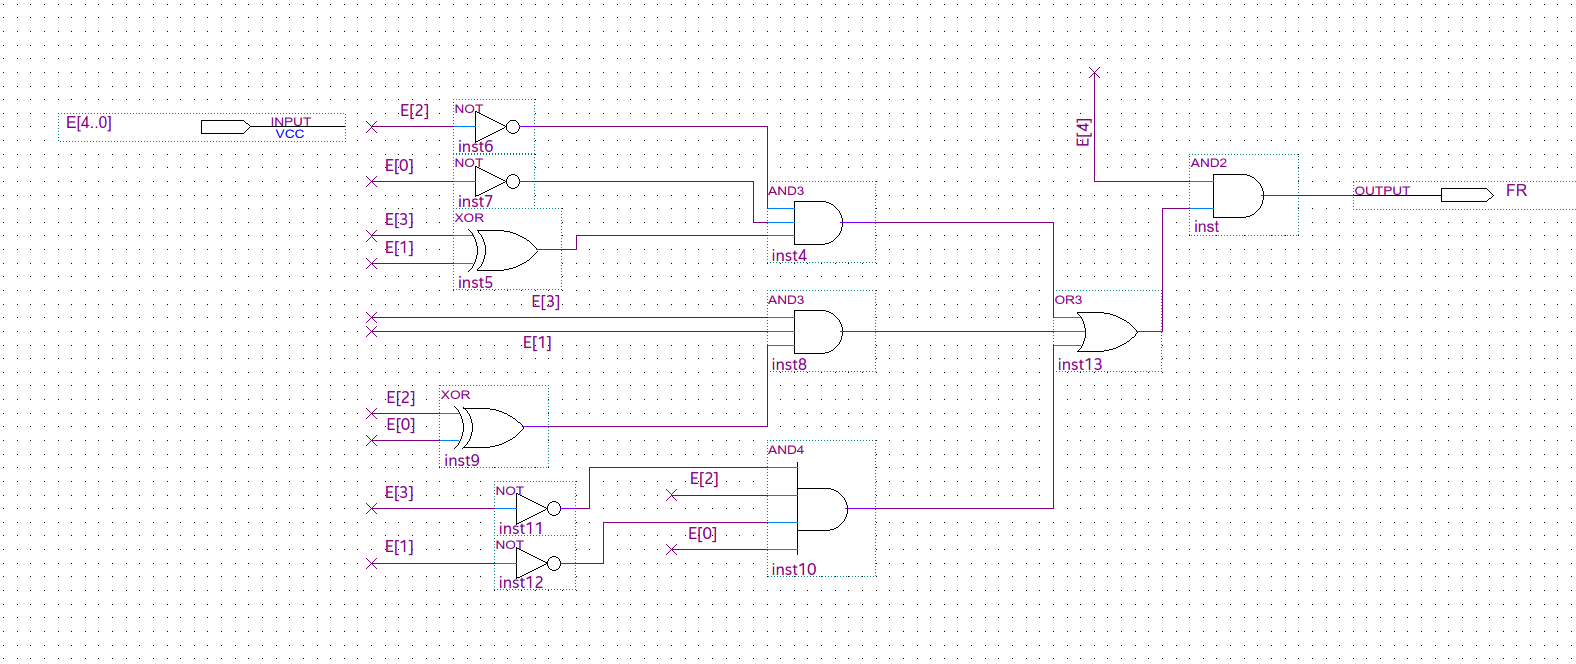
\includegraphics[width=\textwidth]{a_fr}
  \caption{Implementación de $f_r(cwxyz)$}
  \label{fig:a_fr}
\end{figure}

Para cada uno de los diagramas anteriores, se convirtió en un símbolo, con la 
finalidad de juntar el comportamiento de ambos dentro de un ``módulo 
principal'', el cual se muestra a continuación:
\begin{figure}[H]
  \centering
  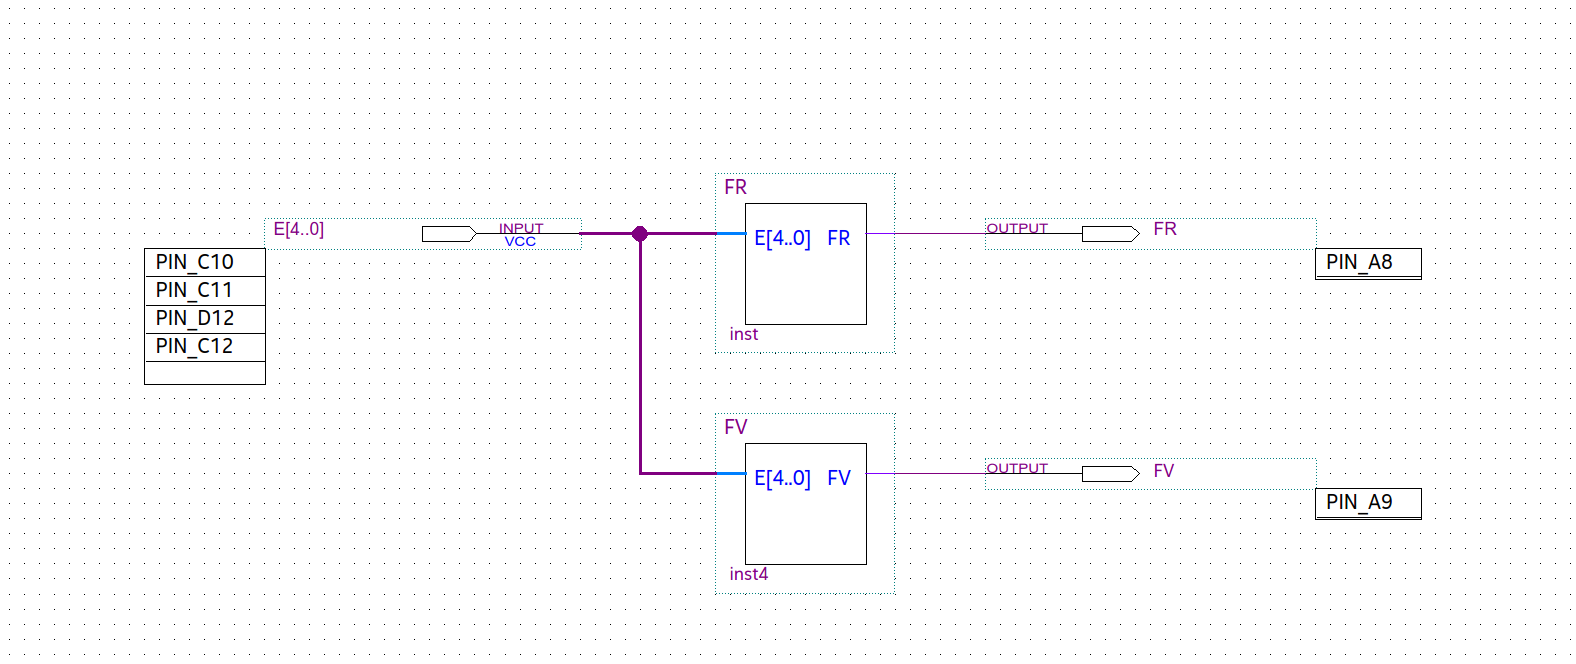
\includegraphics[width=\textwidth]{a_complete}
  \caption{Implementación completa (Sección A)}
  \label{fig:a_complete}
\end{figure}

De igual forma que en las prácticas anteriores, se hizo uso de un archivo 
\textit{University Program VWF} para simular el circuito, el resultado fue el 
siguiente:
\begin{figure}[H]
  \centering
  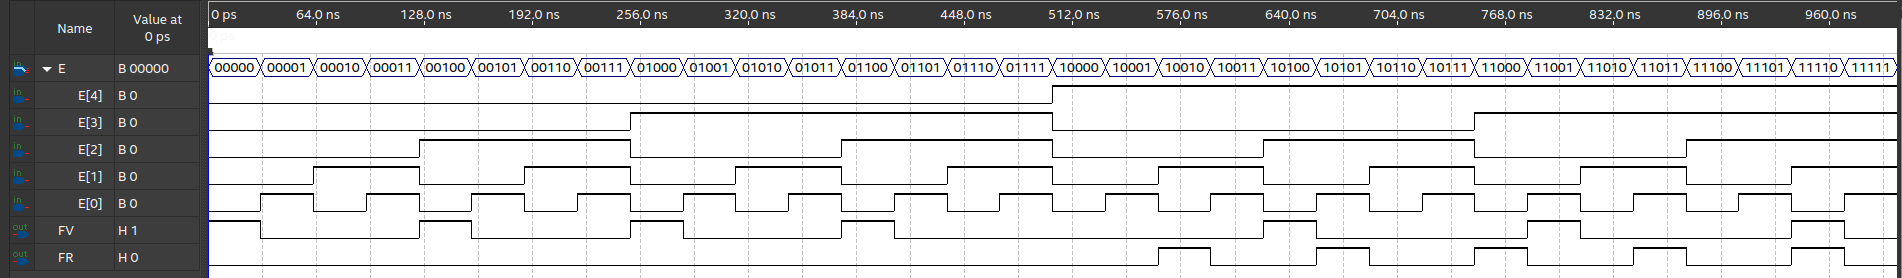
\includegraphics[width=\textwidth]{a_sim}
  \caption{Simulación del sistema (Sección A)}
  \label{fig:a_sim}
\end{figure}

Se puede comprobar que el comportamiento descrito en la Figura \ref{fig:a_sim} 
es el indicado ya que los puntos donde las señales de salida ($f_v$ y $f_r$) 
se activan son justamente los miniterminos planteados en el análisis del 
problema.

\subsection{Ejecución en la FPGA}
Primero, se cargaron los pines correspondientes a través de la ventana 
\textit{Pin Planner}. La asignación fue la misma que se muestra en la Figura 
\ref{fig:a_complete}, donde los pines PIN\_C10, PIN\_C11, PIN\_D12 y PIN\_C12 
son las señales de entrada; mientras que PIN\_A9 es la salida del LED verde y 
PIN\_A8 es la salida del LED rojo.

Posteriormente, se volvió a compilar el proyecto para tomar en cuenta los 
nuevos pines de entrada/salida. Y, finalmente, a través de la ventana 
\textit{Porgrammer}, se cargó el archivo cn exel archivo cn extensión 
\textit{.sof} a la tarjeta de desarrollo \textit{DE10-Lite}.

A continuación, se muestran algunos casos de prueba dentro de la tarjeta. Los 
LED's que simulan la salida son los dos de hasta la derecha: LEDR1 es el LED 
verde y LEDR0 es el LED rojo. Por otra parte, las entradas al sistema son los 
cinco \textit{switch} que se encuentras más a la derecha ---de más 
significativo a menos significativo de izquierda a derecha.
\begin{figure}[H]
  \centering
  \begin{subfigure}[b]{0.45\textwidth}
    \centering
    \caption{Caso de prueba 01100 (12)}
    \label{fig:a_tarj_1}
    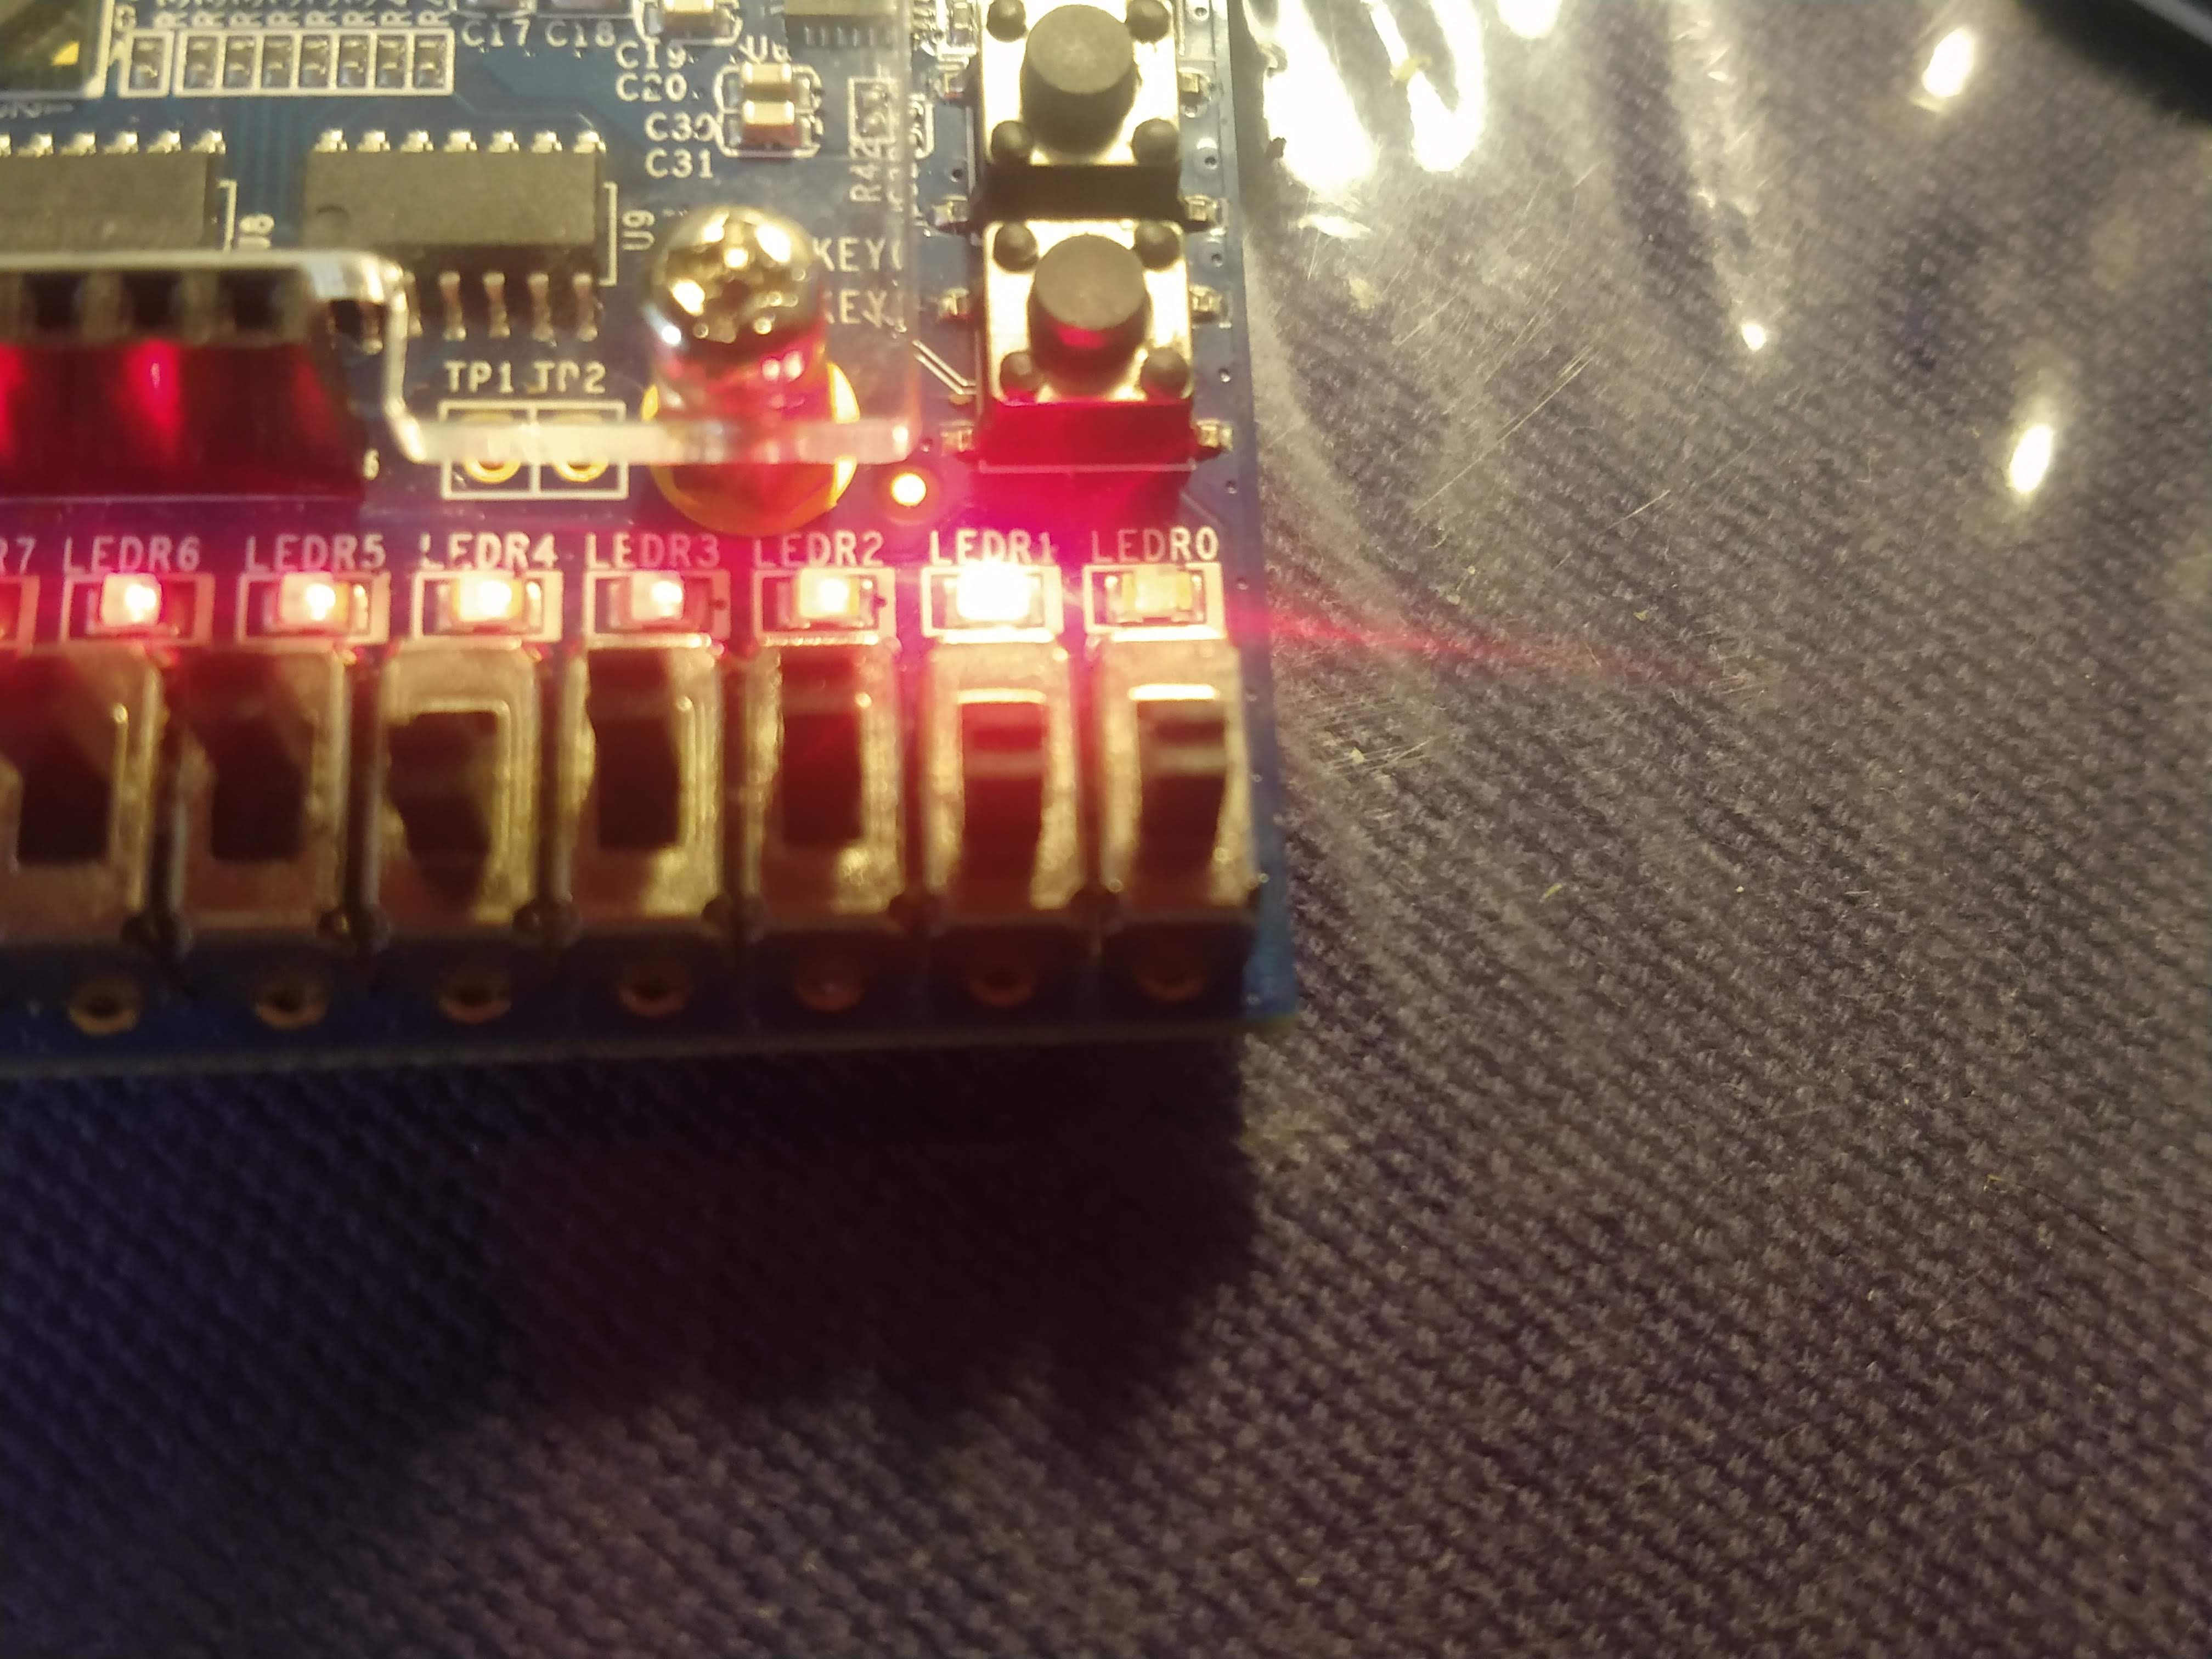
\includegraphics[width=\textwidth]{a_tarj_1}
  \end{subfigure}
  \begin{subfigure}[b]{0.45\textwidth}
    \centering
    \caption{Caso de prueba 10101 (25)}
    \label{fig:a_tarj_2}
    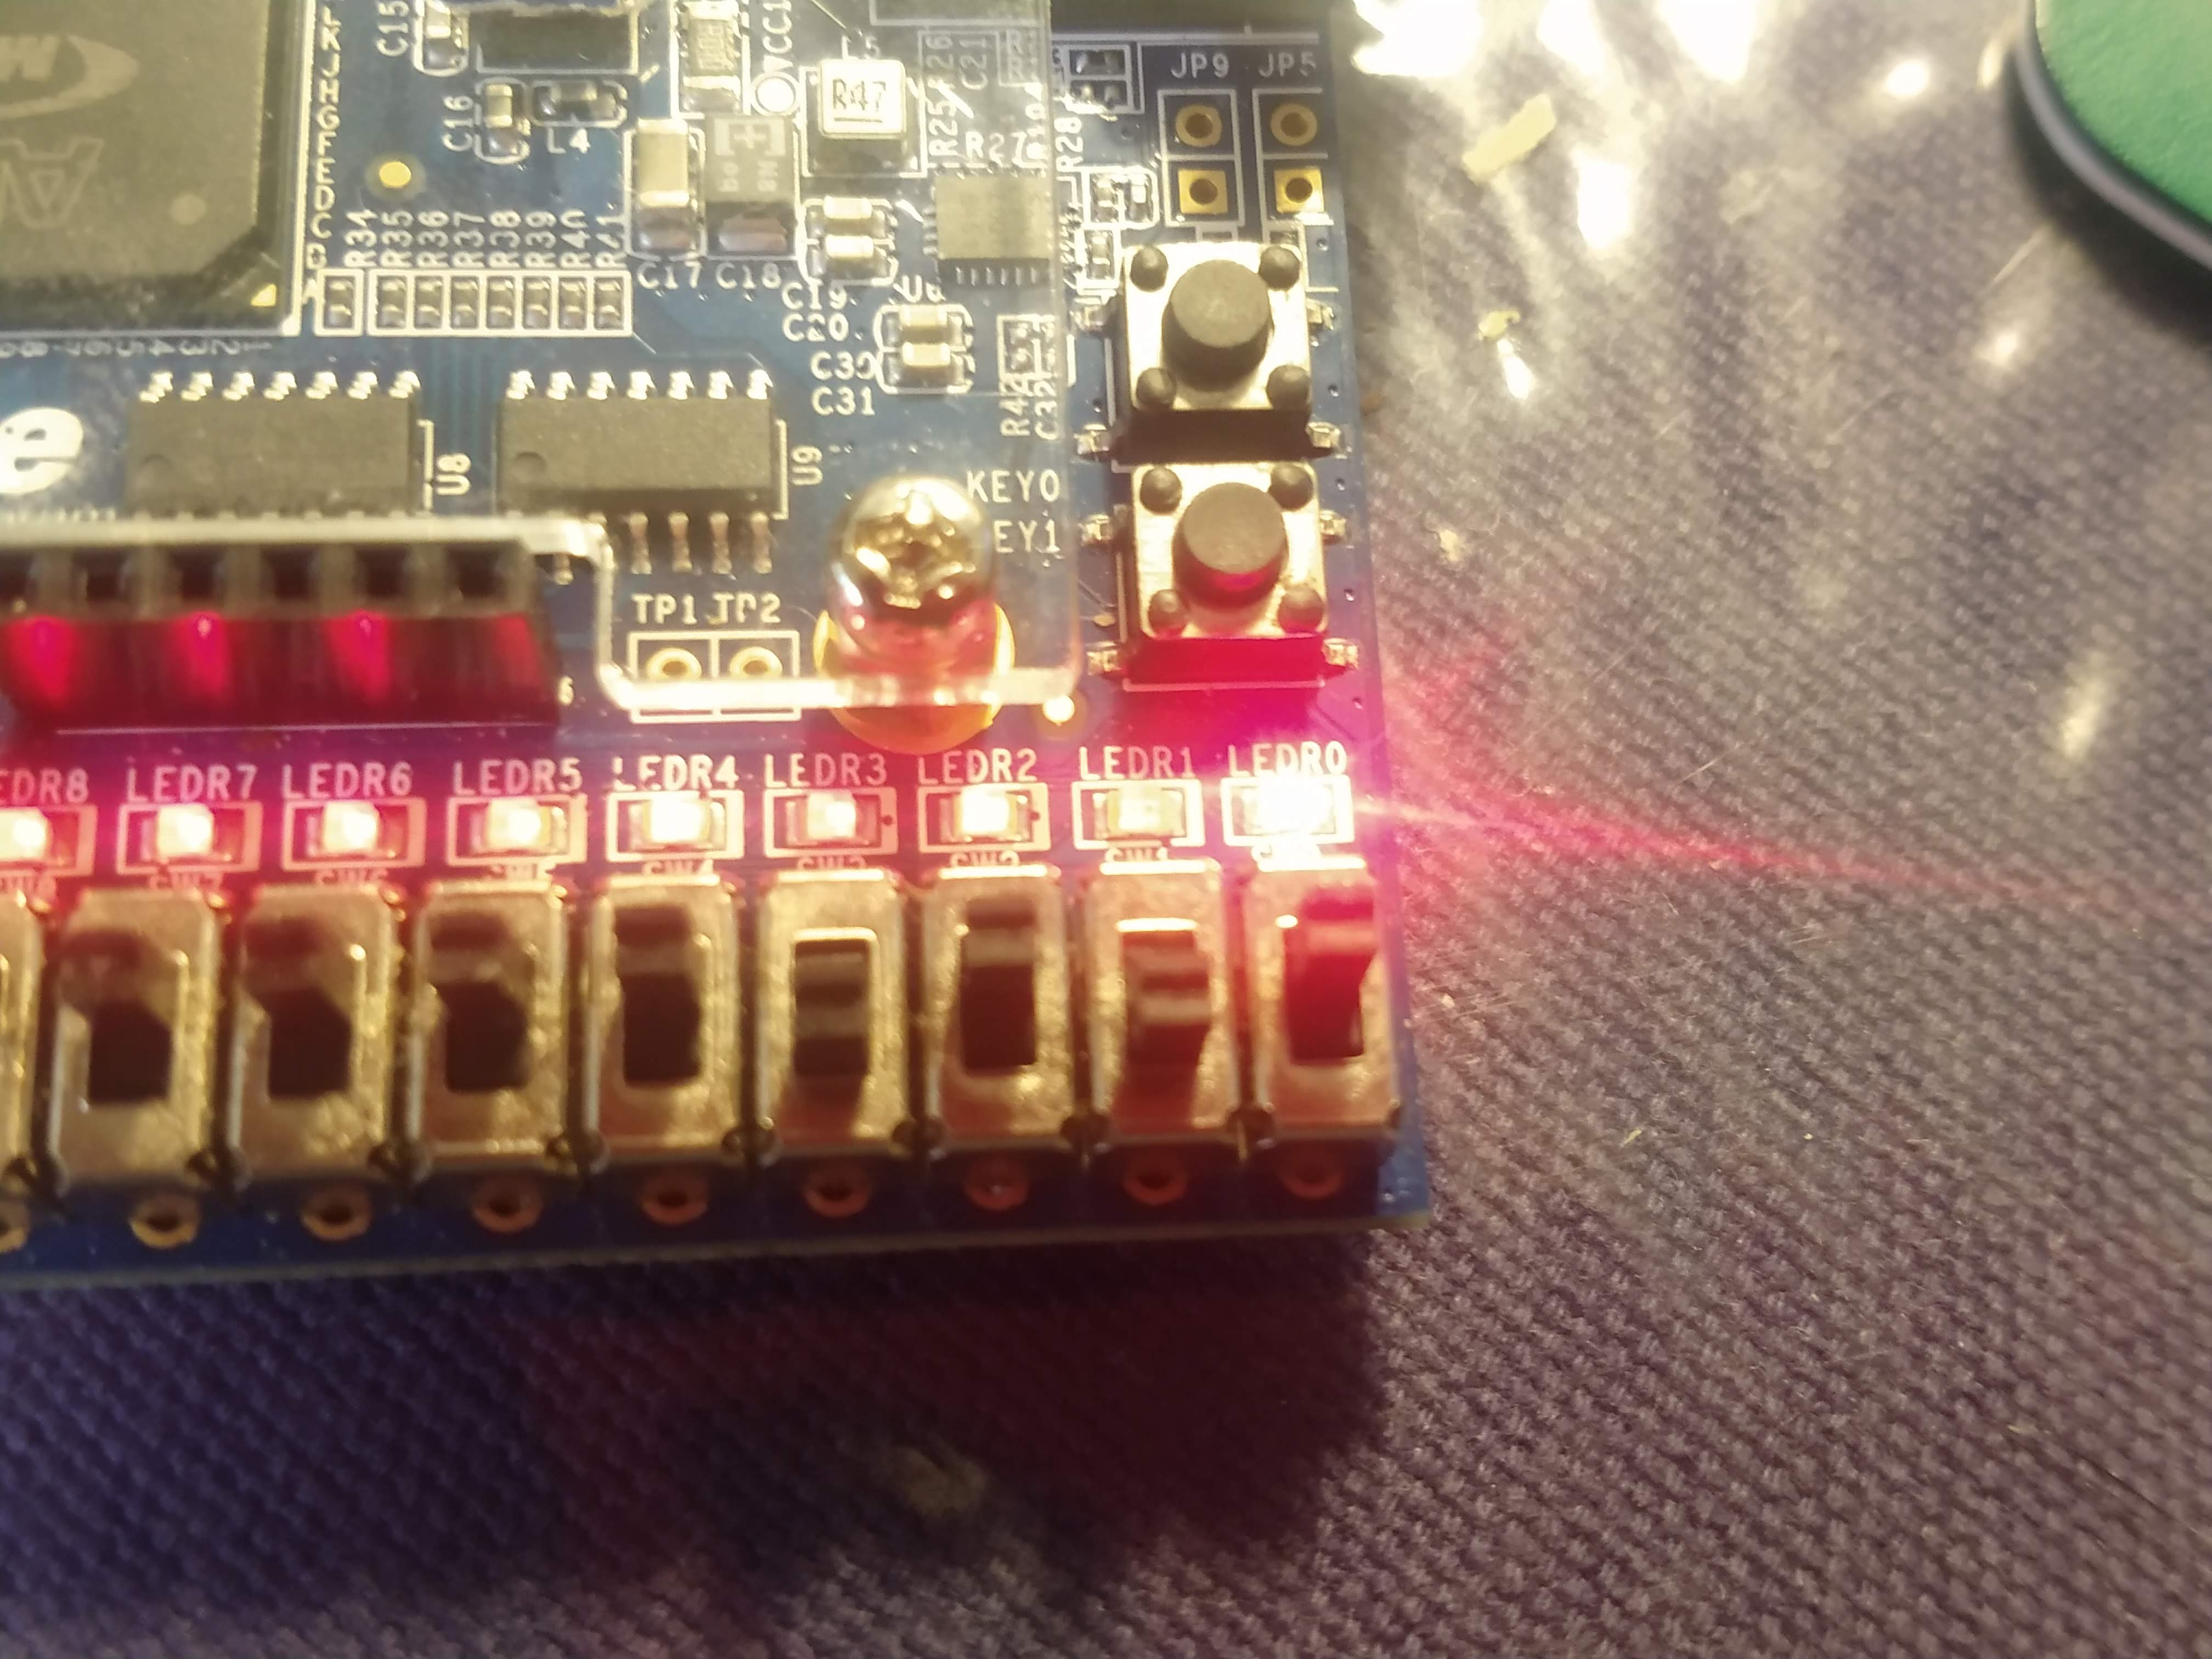
\includegraphics[width=\textwidth]{a_tarj_2}
  \end{subfigure}
  \begin{subfigure}[b]{0.45\textwidth}
    \centering
    \caption{Caso de prueba 11001 (21)}
    \label{fig:a_tarj_3}
    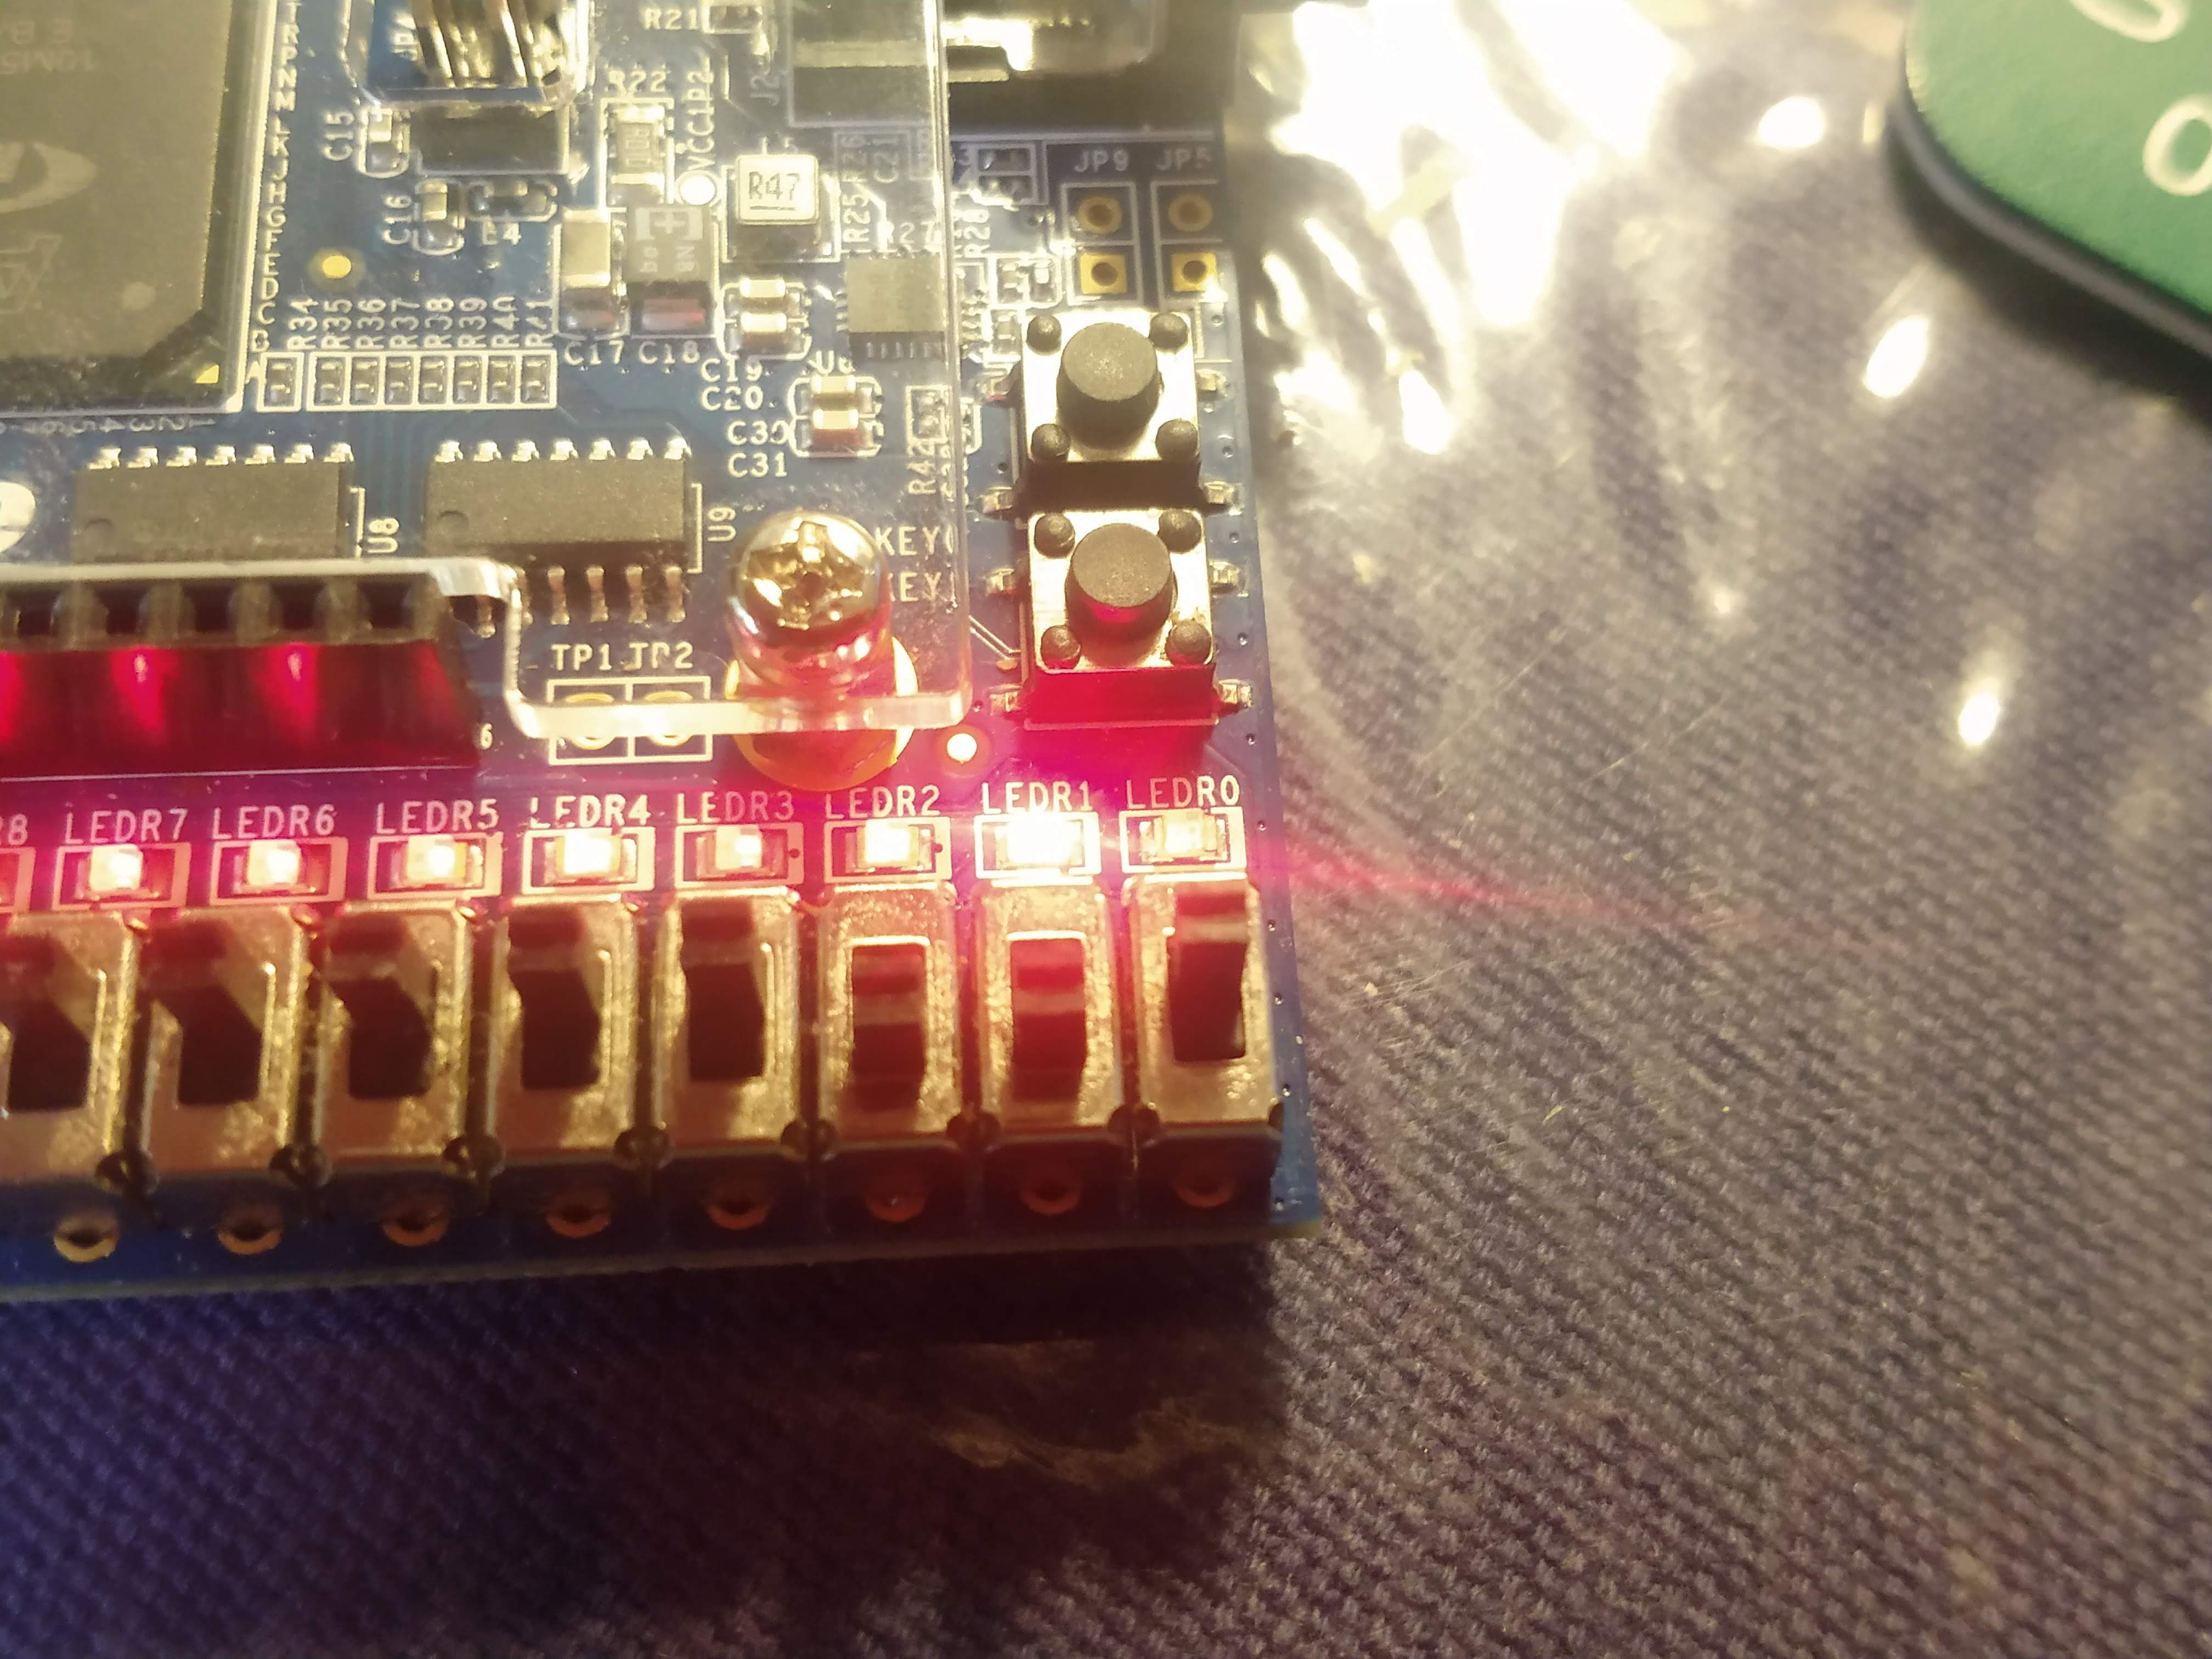
\includegraphics[width=\textwidth]{a_tarj_3}
  \end{subfigure}
  \begin{subfigure}[b]{0.45\textwidth}
    \centering
    \caption{Caso de prueba 11110 (30)}
    \label{fig:a_tarj_4}
    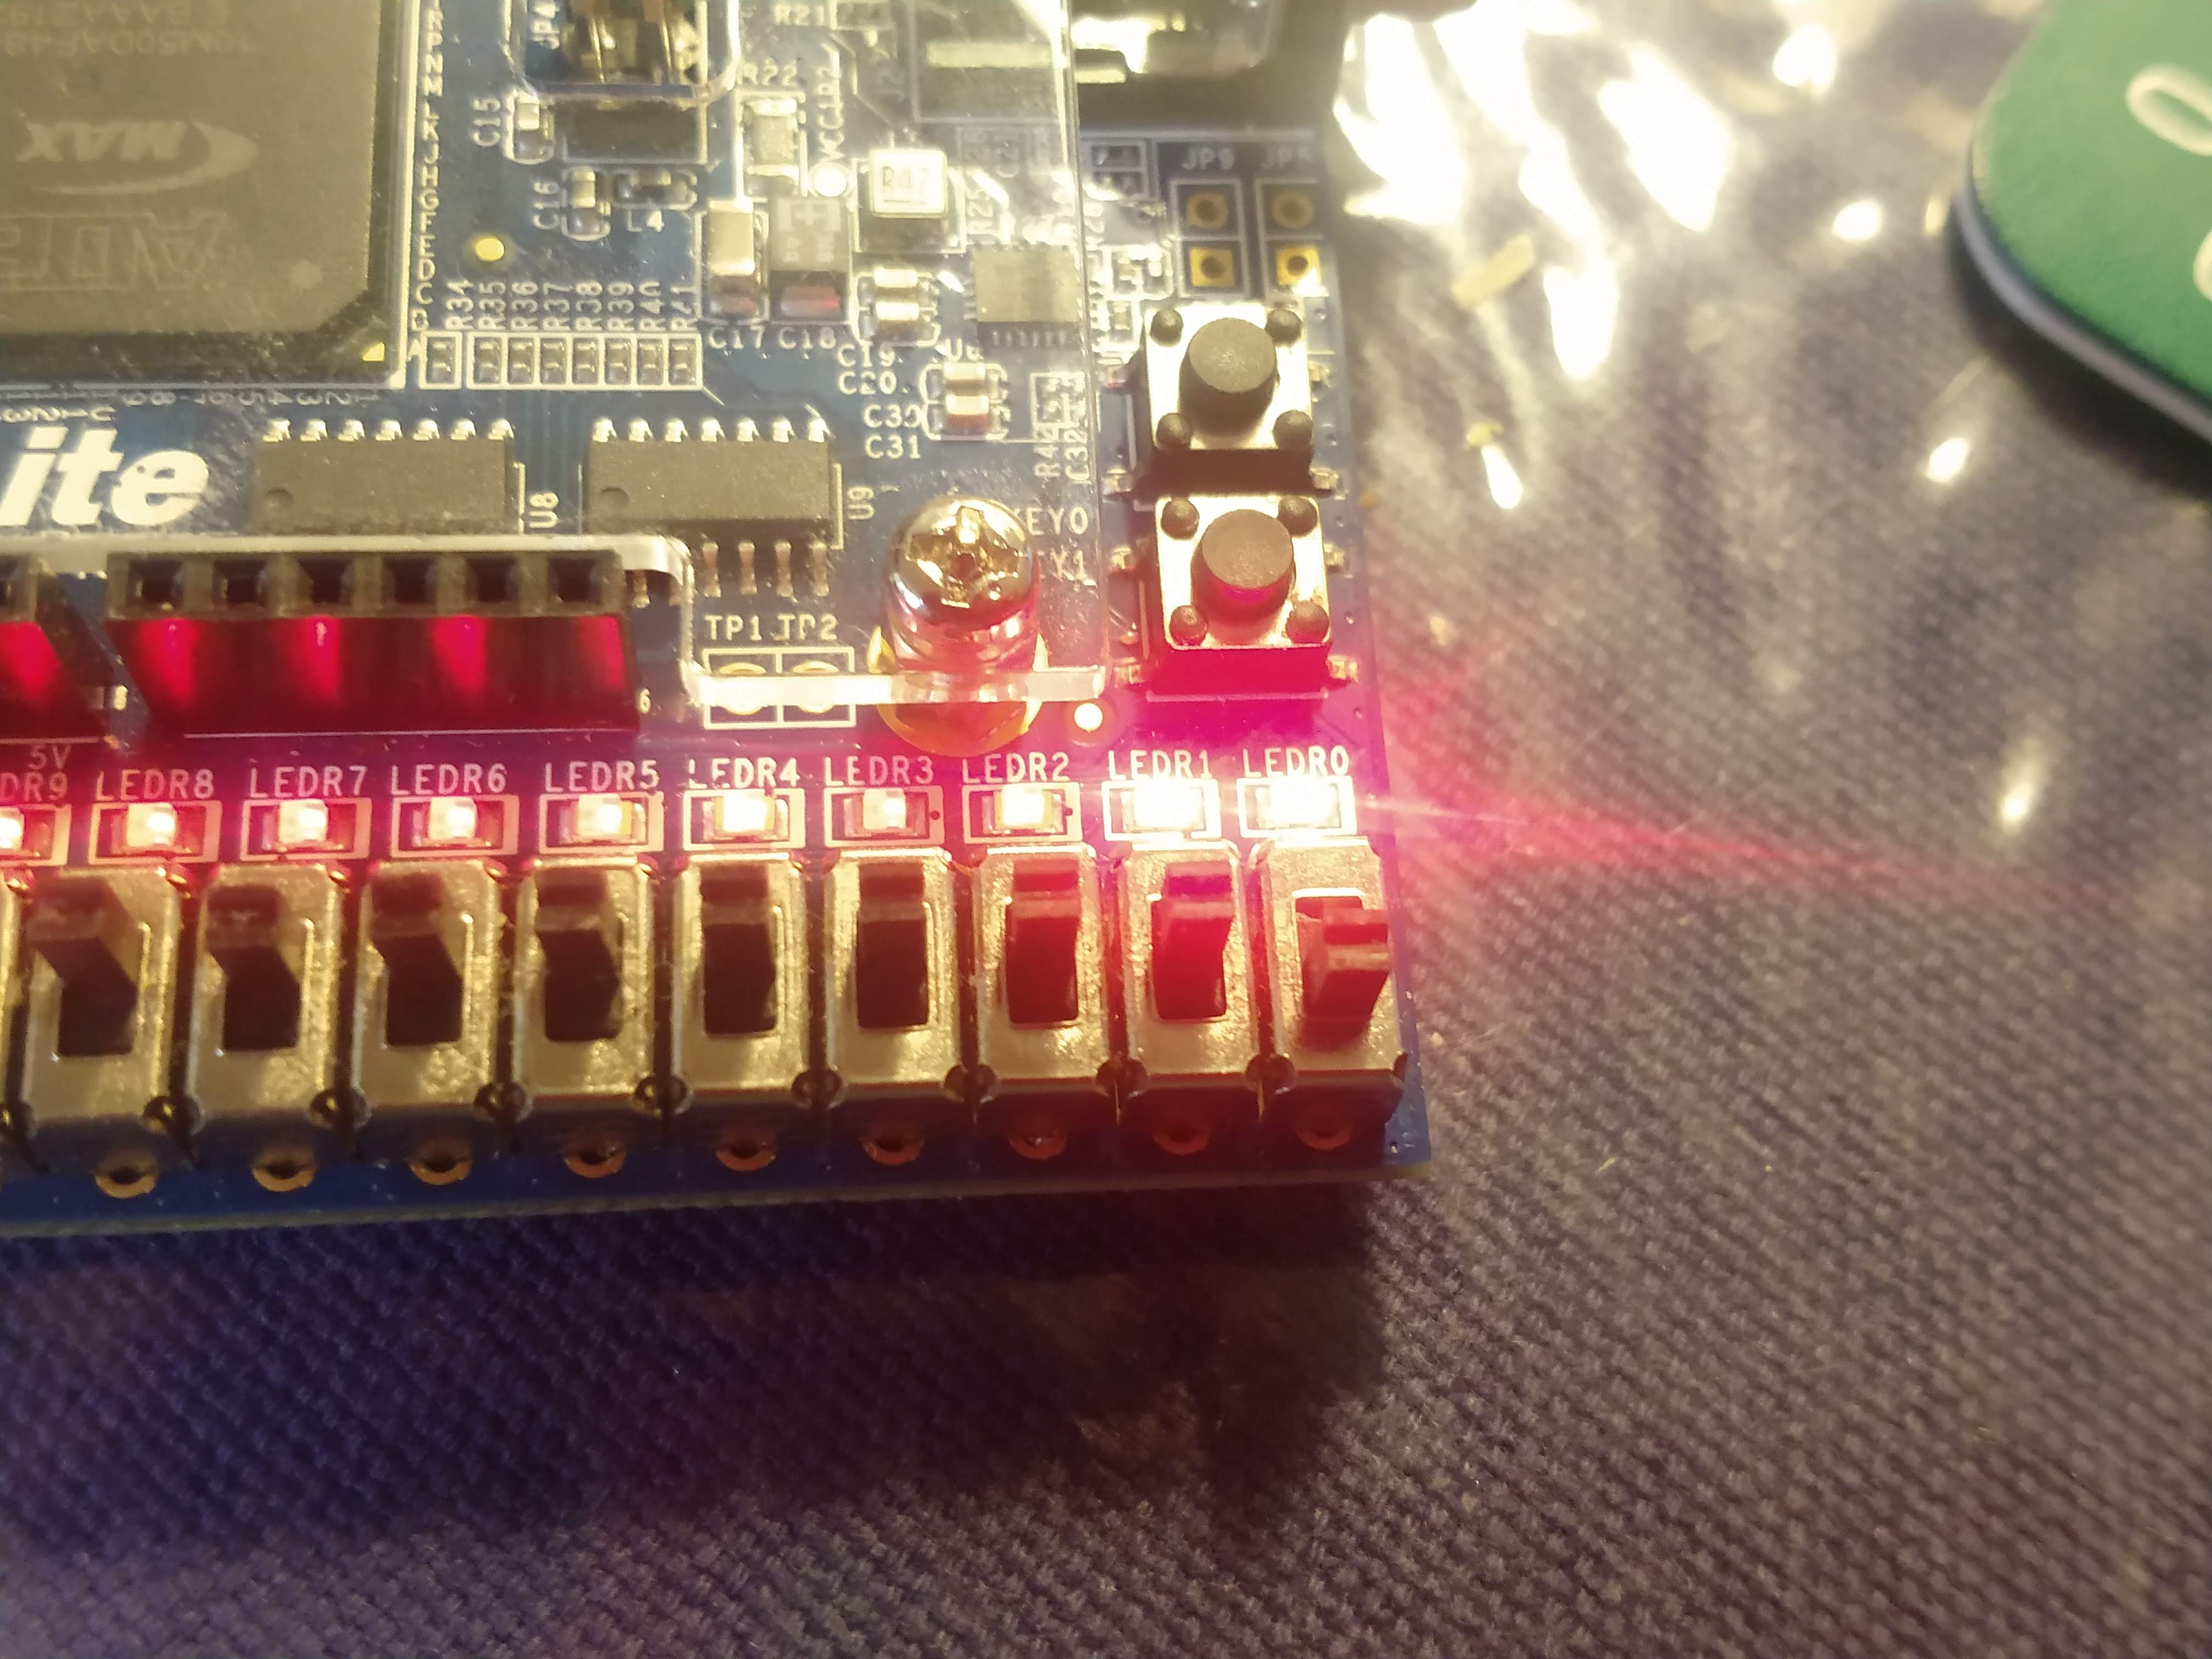
\includegraphics[width=\textwidth]{a_tarj_4}
  \end{subfigure}
  \caption{Casos de prueba (Sección A)}
\end{figure}

Los casos de prueba se comportan según lo esperado:
\begin{itemize}
  \item Para el caso de \ref{fig:a_tarj_1}: El mintérmino 12 prende el LED 
    verde (LED izquierdo).
  \item Para el caso de \ref{fig:a_tarj_2}: El mintérmino 25 prende el LED 
    verde (LED izquierdo).
  \item Para el caso de \ref{fig:a_tarj_3}: El mintérmino 21 prende el LED 
    rojo (LED derecho).
  \item Para el caso de \ref{fig:a_tarj_4}: El mintérmino 30 prende ambos 
    LED's.
\end{itemize}
\end{document}

